\documentclass[aspectratio=169]{beamer}
\usepackage[T1]{fontenc}
\usepackage[utf8]{inputenc}
\usepackage{tikz}
\usepackage{tabularx}
\usepackage[font=scriptsize]{caption}
\usepackage{multirow}
\captionsetup[figure]{labelformat=empty}

\usetikzlibrary{tikzmark,shapes,arrows,backgrounds,fit,positioning}
\newcolumntype{C}{>{\centering\arraybackslash}X}
\newcolumntype{R}{>{\raggedleft\arraybackslash}X}

\addtobeamertemplate{navigation symbols}{}
{
	\insertframenumber{}
}

\beamertemplatenavigationsymbolsempty
\setbeamercolor{section in foot}{fg=white, bg=blue}
\setbeamercolor{subsection in foot}{fg=black, bg=white}
\setbeamerfont{footline}{size=\fontsize{6}{6}\selectfont}

\setbeamertemplate{footline}
{
  \leavevmode
  \hbox
  {
    \begin{beamercolorbox}
      [wd=.5\paperwidth,ht=2.5ex,dp=1.125ex,leftskip=.3cm,rightskip=.3cm]{subsection in foot}
    \end{beamercolorbox}
    
    \begin{beamercolorbox}
      [wd=.5\paperwidth,ht=2.5ex,dp=1.125ex,leftskip=.3cm,rightskip=.3cm plus1fil]{subsection in foot}
      \hfill
      \insertframenumber
      %\insertframenumber\,/\,\inserttotalframenumber
    \end{beamercolorbox}
  }
}


\title{UUB Charge and Peak histograms}
\author{
  Mauricio Su\'arez Dur\'an and Ioana~C.~Mari\c{s}
}
\institute{IIHE-ULB}

\titlegraphic{
  \begin{figure}[h]
    \centering
   %
\includegraphics[width=5cm]{ulbLogo2.png}
    \hspace*{8.cm}
    
\includegraphics[width=5.5cm]{iihe.jpeg}
  \end{figure}
}

\begin{document}
\begin{frame}
  \titlepage
\end{frame}


\begin{frame}
	\frametitle{UUB Charge and Peak histograms}
	\begin{itemize}
		\item Station studied: 863 1222 1219 1211 1740 1743 1221 1223 1217 1747 1741 1745 1818 1851 1729 1735 1746 1819 1791
		\item Data from CDAS.
		\item {\underline {Software CDAS, pre-production version.}}
	\end{itemize}
	\centering
	\includegraphics[width=.45\textwidth]{mapStations.pdf}
\end{frame}


\begin{frame}
  \frametitle{Understanding the sampling}
  \begin{figure}
    \centering
    \begin{tabularx}{\textwidth}{CC}
      \begin{tabular}{l}
        \includegraphics[width=.45\textwidth]{../plots/originalPulseGapNote199-004.png}
      \end{tabular}
      &
      \begin{tabular}{l}
        \includegraphics[width=.45\textwidth]{../plots/samplingPulseGapNote199-004.png}
      \end{tabular}
      \\
      \begin{tabular}{l}
        \includegraphics[width=.45\textwidth]{../plots/samplingDigiPulseGapNote199-004.png}
      \end{tabular}
      &
      \footnotesize
      \begin{tabular}{c|c|c|c}
        {} & Orig. Pulse & $2^{10}$ at $25$\,ns & $2^{12}$ at $8.33$\,ns \\ \hline
        Area & $111.85$\,pC & $105.30$\,pC & $109.88$\,pC \\
        Peak & $69.01$\,mV & $64.35$\,mV & $68.60$\,mV \\
        AoP & $1.62$\,nF & $1.64$\,nF & $1.61$\,nF \\ 
        \multicolumn{4}{l}{From FADC to Amplitud (mV):} \\
        \multicolumn{4}{l}{$1$\,FADC = $2000.$\,mV / $2^{n}$, where $n$ takes 10 or 12.} \\
        \multicolumn{4}{l}{} \\
        \multicolumn{4}{l}{From FADC to Charge (pC):} \\
        \multicolumn{4}{l}{Q $= \frac{(\Delta t\,\mathrm{ns})(2000.\,\mathrm{mV} / 2^{n})}{50.\,\Omega} \sum{n_i}
        = \sum{n_i}$\,pC}
      \end{tabular}
    \end{tabularx}
  \end{figure}
\end{frame}


\begin{frame}
  \frametitle{AoP ratio expected for $25.00$\,ns / $8.33$\,ns}
  $ \frac{ \mathrm{AoP}^{25} } {\mathrm{AoP}^{8.33}}
  = \frac{1.64\,\mathrm{nF}}{1.61\,\mathrm{nF}} = 1.02$;
  How is this ratio for an artifial sample of $10^4$ pulses?

  \begin{figure}
    \centering
    \begin{tabularx}{\textwidth}{CC}
      \begin{tabular}{l}
        \includegraphics[width=.45\textwidth]{../plots/artifitialPulses.pdf}
      \end{tabular}
      &
      \footnotesize
      \begin{tabular}{c|c|c|c}
        {} & $25$\,ns & $8.33$\,ns & $1.0$\,ns \\ \hline
        Area & $105.11$\,pC & $110.23$\,pC & $111.87$\,pC \\
        Peak & $65.59$\,mV & $68.72$\,mV & $69.03$\,mV \\
        AoP & $1.60$\,nF & $1.60$\,nF & $ 1.62$ \\ \hline
        Ratio AoP & \multicolumn{3}{c}{1.00} \\
        \multicolumn{4}{l}{} \\
        \multicolumn{4}{l}{The AoP is the same for both sampling.} \\
        \multicolumn{4}{l}{8.33's Area and Peak bigger than 25.'s ones.}
      \end{tabular}
      \\
      \begin{tabular}{l}
        \includegraphics[width=.45\textwidth]{../plots/samplingDigiPkHistos.pdf}
      \end{tabular}
      &
      \begin{tabular}{l}
        \includegraphics[width=.45\textwidth]{../plots/samplingDigiChHistos.pdf}
      \end{tabular}
    \end{tabularx}
  \end{figure}
\end{frame}


\begin{frame}
  \frametitle{What to expect for different HV ($1.5*$P0)?}
  \begin{figure}
    \centering
    \begin{tabularx}{\textwidth}{CC}
      \begin{tabular}{l}
        \includegraphics[width=.5\textwidth]{../plots/artifitialPulsesAmp.pdf}
      \end{tabular}
      &
      \footnotesize
      \begin{tabular}{c|c|c|c}
        {} & $25.00$\,ns & $8.33$\,ns & $1.0$\,ns \\ \hline
        Area & $162.50$\,pC & $169.57$\,pC & $167.79$\,Pc \\
        Peak & $98.37$\,mV & $103.06$\,mV & $103.55$\,mV \\
        AoP & $1.65$\,nF & $1.65$\,nF & $1.62$\,nF\\ \hline
        Ratio AoP & \multicolumn{3}{c}{1.00} \\
        \multicolumn{4}{c}{} \\
        \multicolumn{4}{l}{Here, the change of amplitude causes} \\
        \multicolumn{4}{l}{a different of $\sim3$\,\% in the AoP value.} \\
        \multicolumn{4}{l}{8.33's Area and Peak bigger than 25.'s ones.}
      \end{tabular}
      \\
      \begin{tabular}{l}
        \includegraphics[width=.48\textwidth]{../plots/samplingiDigiPkHistosAmp.pdf}
      \end{tabular}
      &
      \begin{tabular}{l}
        \includegraphics[width=.48\textwidth]{../plots/samplingDigiChHistosAmp.pdf}
      \end{tabular}
    \end{tabularx}
  \end{figure}
\end{frame}


\begin{frame}
  \frametitle{Checking AoP for Station 863}
  \begin{figure}
    \centering
    \begin{tabularx}{\textwidth}{CC}
      \begin{tabular}{l}
        \includegraphics[width=.45\textwidth]{../plots/uububAoPtimeHbPMT1St863.png}
      \end{tabular}
      &
      \begin{tabular}{l}
        \includegraphics[width=.45\textwidth]{../plots/uububAoPtimeHbPMT2St863.png}
      \end{tabular}
      \\
      \begin{tabular}{l}
        \includegraphics[width=.45\textwidth]{../plots/uububAoPtimeHbPMT3St863.png}
      \end{tabular}
      &
      How good is the fit?
    \end{tabularx}
  \end{figure}
\end{frame}

\begin{frame}
  \frametitle{Checking for UUB {\huge $\chi^2/$ndf} Station 863}
  \begin{figure}
    \centering
    \includegraphics[width=.91\textwidth]{../plots/uubPeakChisHbSt863PMTs.pdf}
  \end{figure}
  \footnotesize
  All fits with $\chi^2/\mathrm{ndf} > 50$ were counted as $49$.
\end{frame}

\begin{frame}
  \frametitle{Checking for UB {\huge $\chi^2/$ndf} Station 863}
  \begin{figure}
    \centering
    \includegraphics[width=.91\textwidth]{../plots/ubPeakChisHbSt863PMTs.pdf}
  \end{figure}
  \footnotesize
  All fits with $\chi^2/\mathrm{ndf} > 50$ were counted as $49$.
\end{frame}

\begin{frame}
  \frametitle{Checking Peak and Charge for Station 863}
  \begin{figure}
    \centering
    \begin{tabularx}{\textwidth}{CC}
      \begin{tabular}{l}
        \includegraphics[width=.47\textwidth]{../plots/uubPeaktimeHbSt863PMTs.png}
      \end{tabular}
      &
      \begin{tabular}{l}
        \includegraphics[width=.47\textwidth]{../plots/uubChargetimeHbSt863PMTs.png}
      \end{tabular}
      \\
    \end{tabularx}
  \end{figure}

  \begin{center}
    \small
    \begin{tabular}{|c|c|c|c|c|c|c|}
      \hline
      \multirow{2}{*}{} & \multicolumn{2}{c|}{PMT1} & \multicolumn{2}{c|}{PMT2} & \multicolumn{2}{c|}{PMT3} \\ \cline{2-7}
        & UB & UUB & UB & UUB & UB & UUB \\ \hline
      Area & $121.43$\,pC & $102.84$\,pC & $104.41$\,pC & $122.81$\,pC & $146.26$\,pC & $107.43$\,pC \\ \hline
      Peak & $71.15$\,mV  & $72.28$\,mV  & $52.51$\,mV  & $86.98$\,mV  & $52.51$\,mV  & $75.26$\, mV\\  \hline
      AoP  & $1.71$\,nF   & $1.42$\,nF   & $1.99$\,nF   & $1.41$\,nF   & $2.79$\,nF   & $1.43$\,nF \\ \hline
    \end{tabular}
    \\
    \vspace{0.5cm}
    May be a differente HV?
  \end{center}

\end{frame}


\begin{frame}
  \frametitle{Checking for St. 863's HV}
  Data from /pbs/throng/pauger/DATA/Raid/monit/ and readed with TSDMonCal.h
  \centering
  %\vspace{0.5cm}
  \includegraphics[width=.8\textwidth]{../plots/uubHVSt863.png}
  \\
  \small
  fPMV[pmt] and UPMV[pmt] are not the correct variables to check this?
  \\
  Which are the correct ones?
\end{frame}

\begin{frame}
  \frametitle{Checking for St. 863's HV}
  From http://mon.auger.uni-wuppertal.de/pro/SD/LS/Monitoring.php?LSId=863
  \begin{figure}
    \centering
    \begin{tabularx}{\textwidth}{CC}
      \includegraphics[width=.42\textwidth]{../plots/uububHv863pmt1web.png}
      &
      \includegraphics[width=.42\textwidth]{../plots/uububHv863pmt2web.png}
    \end{tabularx}
  \end{figure}
  \begin{center}
    \begin{tabular}{l}
      \includegraphics[width=.42\textwidth]{../plots/uububHv863pmt3web.png}
    \end{tabular}
  \end{center}
\end{frame}


\begin{frame}
  \frametitle{Checking AoP for Station 1740}
  \begin{figure}
    \centering
    \begin{tabularx}{\textwidth}{CC}
      \begin{tabular}{l}
        \includegraphics[width=.45\textwidth]{../plots/uububAoPtimeHbPMT1St1740.png}
      \end{tabular}
      &
      \begin{tabular}{l}
        \includegraphics[width=.45\textwidth]{../plots/uububAoPtimeHbPMT2St1740.png}
      \end{tabular}
      \\
    \end{tabularx}
  \end{figure}

  \begin{center}
    \begin{tabular}{l}
      \includegraphics[width=.45\textwidth]{../plots/uububAoPtimeHbPMT3St1740.png}
    \end{tabular} 
  \end{center}
\end{frame}


\begin{frame}
  \frametitle{Checking for UUB {\huge $\chi^2/$ndf} Station 1740}
  \begin{figure}
    \centering
    \includegraphics[width=.91\textwidth]{../plots/uubPeakChisHbSt1740PMTs.pdf}
  \end{figure}
  \footnotesize
  All fits with $\chi^2/\mathrm{ndf} > 50$ were counted as $49$.
\end{frame}

\begin{frame}
  \frametitle{Checking for UB {\huge $\chi^2/$ndf} Station 1740}
  \begin{figure}
    \centering
    \includegraphics[width=.91\textwidth]{../plots/ubPeakChisHbSt1740PMTs.pdf}
  \end{figure}
  \footnotesize
  All fits with $\chi^2/\mathrm{ndf} > 50$ were counted as $49$.
\end{frame}


\begin{frame}
  \frametitle{Checking Area and Peak for Station 1740}
  \begin{figure}
    \centering
    \begin{tabularx}{\textwidth}{CC}
      \begin{tabular}{l}
        \includegraphics[width=.45\textwidth]{../plots/uubPeaktimeHbSt1740PMTs.png}
      \end{tabular}
      \begin{tabular}{l}
        \includegraphics[width=.45\textwidth]{../plots/uubChargetimeHbSt1740PMTs.png}
      \end{tabular}
    \end{tabularx}
    \small
    \begin{tabular}{|c|c|c|c|c|c|c|}
      \hline
      \multirow{2}{*}{} & \multicolumn{2}{c|}{PMT1} & \multicolumn{2}{c|}{PMT2} & \multicolumn{2}{c|}{PMT3} \\ \cline{2-7}
      & UB & UUB & UB & UUB & UB & UUB \\ \hline
      Area & $96.21$\,pC  & $120.27$\,pC & $124.50$\,pC & $112.60$\,pC & $138.46$\,pC & $108.38$\,pC \\ \hline
      Peak & $56.60$\,mV  & $86.19$\,mV  & $74.15$\,mV  & $81.86$\,mV  & $74.15$\,mV  & $78.34$\, mV\\  \hline
      AoP  & $1.67$\,nF   & $1.40$\,nF   & $1.68$\,nF   & $1.34$\,nF   & $1.87$\,nF   & $1.38$\,nF \\ \hline
    \end{tabular}
  \end{figure}
\end{frame}


\begin{frame}
  \frametitle{Checking for St. 1740's HV}
  Data from /pbs/throng/pauger/DATA/Raid/monit/ and readed with TSDMonCal.h
  \centering
  \vspace{0.5cm}

  \includegraphics[width=.8\textwidth]{../plots/uubHVSt1740.png}
\end{frame}

\begin{frame}
  \frametitle{Checking for St. 1740's HV}
  From http://mon.auger.uni-wuppertal.de/pro/SD/LS/Monitoring.php?LSId=1740
  \begin{figure}
    \centering
    \begin{tabularx}{\textwidth}{CC}
      \includegraphics[width=.42\textwidth]{../plots/uububHv1740pmt1web.png}
      &
      \includegraphics[width=.42\textwidth]{../plots/uububHv1740pmt2web.png}
    \end{tabularx}
  \end{figure}

  \begin{center}
    \begin{tabular}{c}
      \includegraphics[width=.42\textwidth]{../plots/uububHv1740pmt3web.png}
    \end{tabular}
  \end{center}
\end{frame}

\begin{frame}
  \frametitle{Checking for Peak for all Stations}
  \centering
  \includegraphics[width=.8\textwidth]{../plots/uubPeaktimeHbAllSt0PMT1.png}
\end{frame}

\begin{frame}
  \frametitle{Checking for Peak for all Stations}
  \centering
  \includegraphics[width=.8\textwidth]{../plots/uubPeaktimeHbAllSt1PMT1.png}
\end{frame}


%\begin{frame}
%  \frametitle{Back-up}
%\end{frame}
%
%\begin{frame}
%  \frametitle{A/P}
%  \begin{figure}
%    \centering
%    \begin{tabularx}{\textwidth}{CC}
%      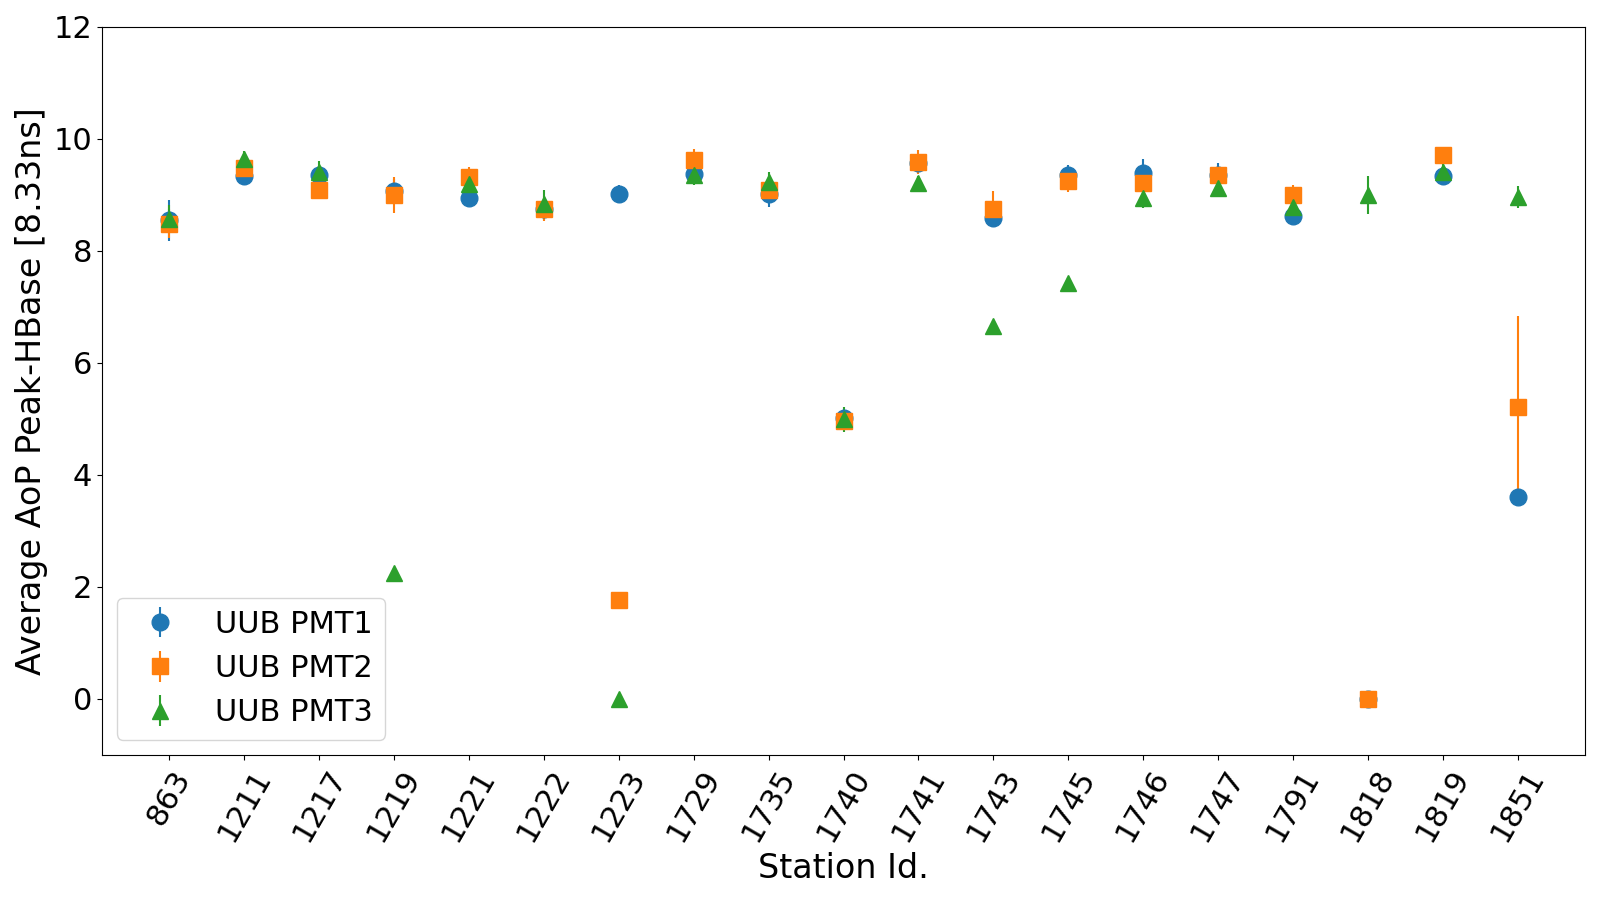
\includegraphics[width=.45\textwidth]{../plots/uubAoPHbasePMTs.png}
%      &
%      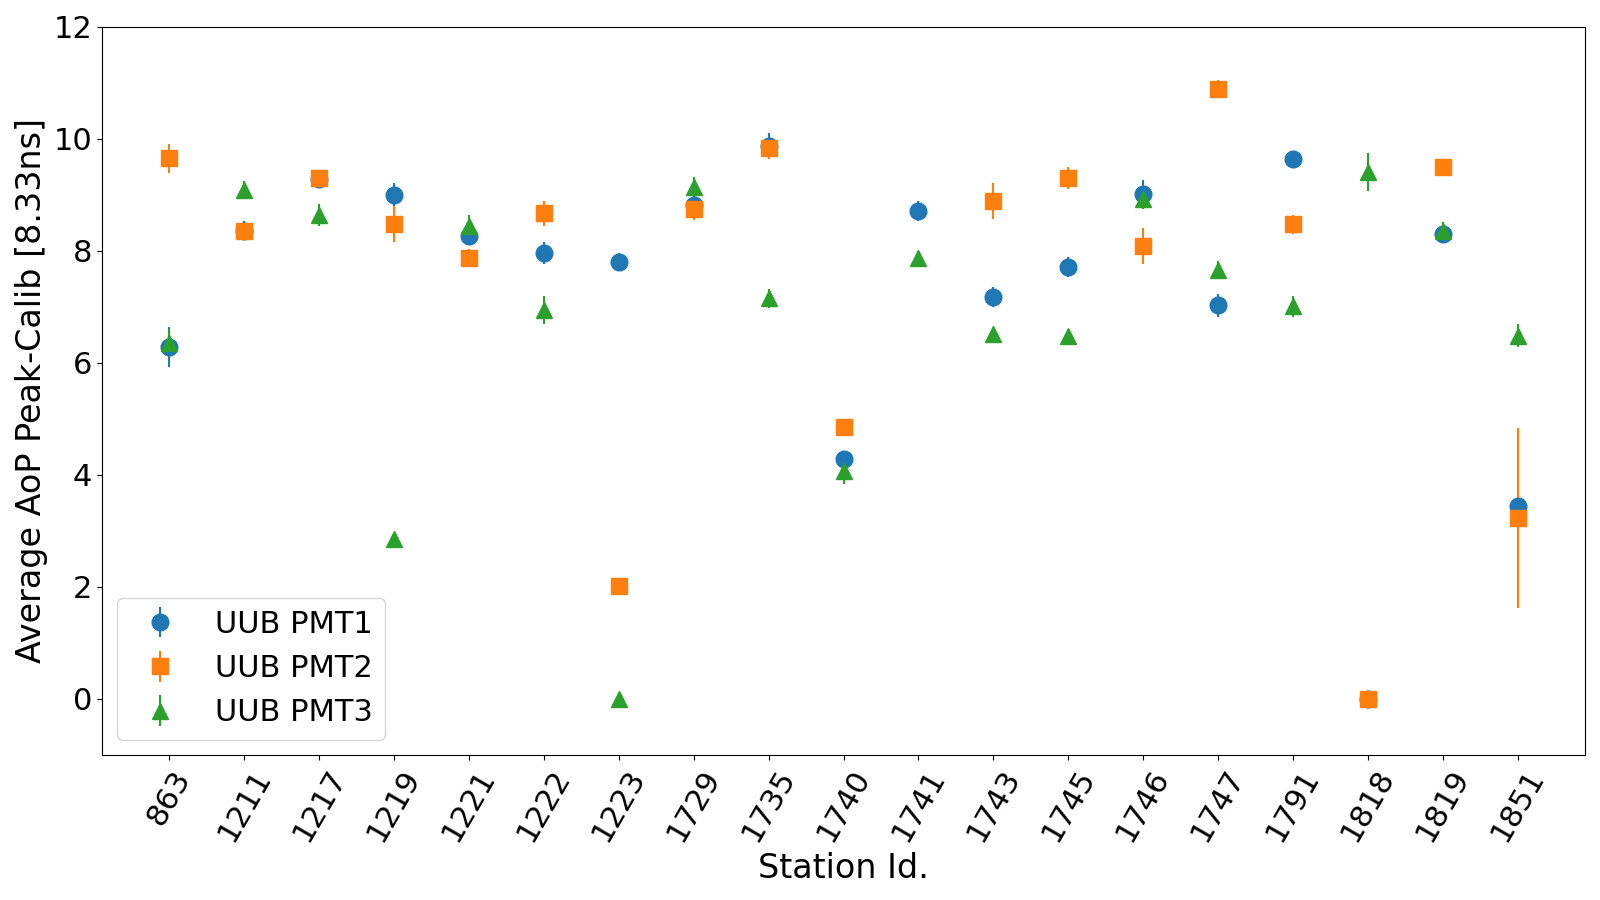
\includegraphics[width=.45\textwidth]{../plots/uubAoPCalibPMTs.png}
%      \\
%      \includegraphics[width=.45\textwidth]{../plots/ubAoPHbasePMTs.png}
%      &
%      \includegraphics[width=.45\textwidth]{../plots/ubAoPCalibPMTs.png}
%    \end{tabularx}
%  \end{figure}
%  \centering
%  
%\end{frame}
%
%
%\begin{frame}
%  \frametitle{A/P Relative difference for Peak corrections}
%  \begin{figure}
%    PMTs with AoP lower than $4$\,ns for UUB and $2$\,ns for UB are not considered here.
%    \centering
%    \begin{tabularx}{\textwidth}{CC}
%      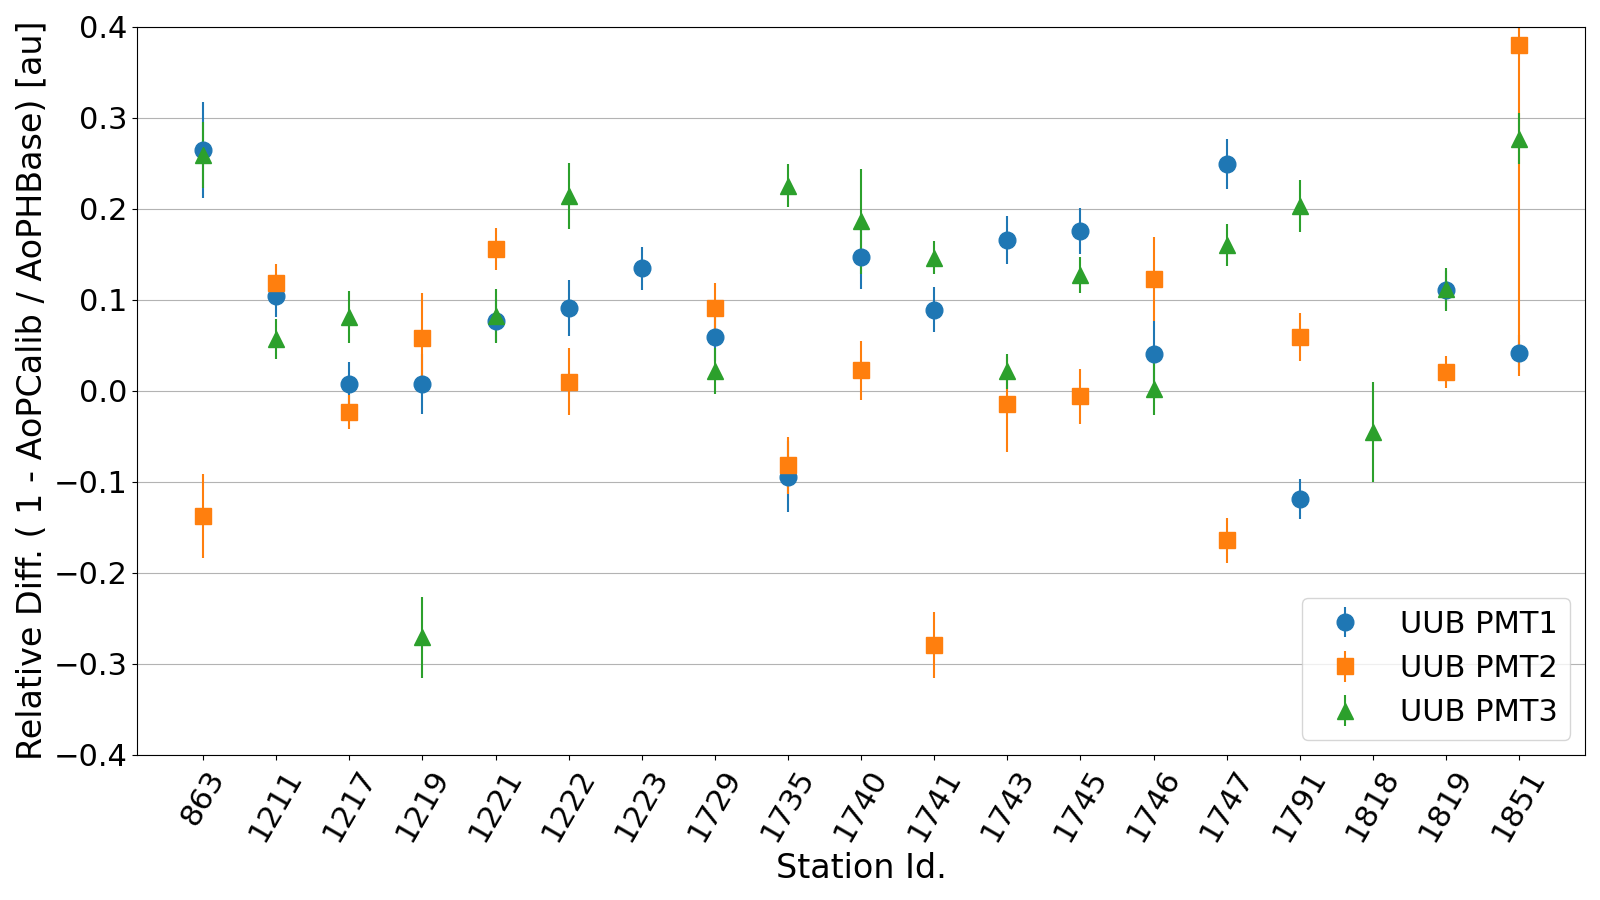
\includegraphics[width=.43\textwidth]{../plots/uubAoPDiffCaHbPMTs.png}
%      &
%      \includegraphics[width=.43\textwidth]{../plots/ubAoPDiffCaHbPMTs.png}
%      \\
%      \includegraphics[width=.43\textwidth]{../plots/aopHbaseUubUbPMTs.png}
%      &
%      \includegraphics[width=.43\textwidth]{../plots/aoCalibUubUbPMTs.png}
%    \end{tabularx}
%  \end{figure}
%\end{frame}
%
%\begin{frame}
%  \frametitle{How well is the fit method works? }
%  {\bf Events-Fitting / Events-total }
%	\begin{figure}
%		\centering
%    \begin{tabularx}{\textwidth}{CC}
%      \begin{tabular}{l}
%        \includegraphics[width=.44\textwidth]{../plots/uubGoodFitEvtnPk.png}
%      \end{tabular}
%      &
%			\begin{tabular}{l}
%				\includegraphics[width=.44\textwidth]{../plots/ubGoodFitEvtnPk.png}
%			\end{tabular}
%			\\
%			\begin{tabular}{l}
%				\includegraphics[width=.44\textwidth]{../plots/uubGoodFitEvtnChPMT.png}
%			\end{tabular} 
%      &
%      \begin{tabular}{l}
%        \includegraphics[width=.44\textwidth]{../plots/ubGoodFitEvtnChPMT.png}
%      \end{tabular}
%		\end{tabularx}
%	\end{figure}
%\end{frame}


\end{document}


%\begin{frame}
%  \begin{figure}
%    \centering
%    \begin{tabularx}{\textwidth}{CC}
%      \begin{tabular}{l}
%        Let's assume a muon pulse as \\
%        exponential function: \\
%        $P(t) = P_{\mathrm{max}}\exp(-t/\tau)$. \\ \\
%        
%        So, the peak takes a value of $P_{\mathrm{max}}$, and \\
%        the integral (A) takes $P_{\mathrm{max}}\tau$. \\ \\
%
%        This means an AoP of $\tau$. \\ \\
%
%        In a digitalized scenario, the $P(t)$ \\
%        takes values each $\Delta t$, which \\
%        means that the $P_{\mathrm{max}}$ will be a value \\
%        between $P(ts)$ and $P(ts + \Delta t)$, where $ts$ \\
%        is the time at which the signal starting. \\ \\
%        Let's say that peak is at $ts$, then \\
%        $P(ts) = P_{\mathrm{max}}\exp(-ts/\tau)$. \\
%      \end{tabular}
%      &
%      \begin{tabular}{l}
%        For the integral: \\
%        $A = \Delta t \sum_{n=1}^{n=\infty} 
%        P_{\mathrm{max}}\exp{-\frac{ts + n\Delta t}{\tau}}$ \\
%
%        $A = P_{\mathrm{max}} \exp^{-ts/\tau} 
%        \frac{\Delta t}{1 - e^{-\Delta t/\tau}}$ \\ \\
%
%        Therefore, we expected an AoP of \\
%        $\mathrm{AoP} = \frac{\Delta t}{1 - e^{-\Delta t/\tau}}$. \\ \\
%
%        If $\Delta t$ goes to zero, so
%        $\mathrm{AoP} = \tau$ 
%      \end{tabular}
%    \end{tabularx}
%  \end{figure}
%\end{frame}
%
%\begin{frame}
%  For UB, AoP takes: \\
%  $\left( \mathrm{AoP}\right)^{\mathrm{UB}} 
%  = \frac{25\,\mathrm{ns}}{1 - e^{-25/\tau}}$\, \\
%  and for UUB, \\
%  $\left( \mathrm{AoP}\right)^{\mathrm{UUB}}
%  = \frac{8.33\,\mathrm{ns}}{1 - e^{-8.33/\tau}}$ \\
%
%  So, 
%  $\frac{ \left( \mathrm{AoP}\right)^{\mathrm{UB}} }
%  { \left(\mathrm{AoP}\right)^{\mathrm{UUB}} }
%  = \frac{25\,\mathrm{ns} \left( 1 - e^{-8.33/\tau} \right)}
%  {8.33\,\mathrm{ns} \left( 1 - e^{-25/\tau} \right)}$ \\
%
%  $\frac{ \left( \mathrm{AoP}\right)^{\mathrm{UB}} }
%  { \left(\mathrm{AoP}\right)^{\mathrm{UUB}} }
%  = 3 \frac{\left( 1 - e^{-8.33/\tau} \right)}{\left( 1 - e^{-25/\tau} \right)} $\\
%
%  Assuming a $\tau=50$\,ns: \\
%  
%  $\frac{ \left( \mathrm{AoP}\right)^{\mathrm{UB}} }
%  { \left(\mathrm{AoP}\right)^{\mathrm{UUB}} }
%  = 3 \frac{0.15}{0.39} = 1.17$ \\
%
%  $\left( \mathrm{AoP}\right)^{\mathrm{UB}} = 1.17 \left(\mathrm{AoP}\right)^{\mathrm{UUB}} $
%
%\end{frame}


%\begin{frame}
%  \frametitle{What to expect for different Mean ($1.5*$P2)?}
%  \begin{figure}
%    \centering
%    \begin{tabularx}{\textwidth}{CC}
%      \begin{tabular}{l}
%        \includegraphics[width=.39\textwidth]{../plots/artifitialPulsesSig.png}
%      \end{tabular}
%      &
%      \small
%      \begin{tabular}{c|c|c|c}
%        {} & $25.00$\,ns & $8.33$\,ns & Rel. Diff. \\ \hline
%        Area & $122.36$\,pC & $177.33$\,pC & $0.31$ \\
%        Peak & $63.59$\,mV & $68.39$\,mV & $0.07$ \\
%        AoP & $1.92$\,nF & $2.59$\,nF & $0.26$\\ \hline
%        Ratio AoP & \multicolumn{3}{c}{0.74}
%      \end{tabular}
%      \\
%      \begin{tabular}{l}
%        \includegraphics[width=.39\textwidth]{../plots/samplingPkHistosSig.png}
%      \end{tabular}
%      &
%      \begin{tabular}{l}
%        \includegraphics[width=.39\textwidth]{../plots/samplingChHistosSig.png}
%      \end{tabular}
%    \end{tabularx}
%  \end{figure}
%\end{frame}

%\begin{frame}
%  \frametitle{Checking for UUB Peak histograms}
%  \begin{figure}
%    \centering
%    \begin{tabularx}{\textwidth}{CC}
%      \begin{tabular}{l}
%        \includegraphics[width=.4\textwidth]{pulseSamples.jpg}
%      \end{tabular}
%      \vspace{0.2cm}
%
%      \begin{tabular}{l}
%        At first approx., we expect a bigger\\
%        UUB VEM-Peak than UB VEM-Peak.\\ \\
%        So, $\frac{1 (\mathrm{VEM}_\mathrm{pk}^{\mathrm{UUB}})} {1 (\mathrm{VEM}_\mathrm{pk}^{\mathrm{UB}})}$
%        $ = \frac{N_\mathrm{pk}^{\mathrm{UUB}}*(0.49\,\mathrm{mV}/8.33\,\mathrm{ns})}
%        {N_\mathrm{pk}^{\mathrm{UB}}*(1.95\,\mathrm{mV}/25\,\mathrm{ns})}$\\ \\
%
%        Where $0.49$\,mV $= 2$\,V$/2^{12}$ and\\ 
%        $1.95$\,mV $= 2$\,V$/2^{10}$, and $N_\mathrm{pk}^{i}$ is the counts\\
%        in FADC, respectively.
%      \end{tabular}
%      &
%      \begin{tabular}{l}
%        This means, if this pulse resprents a VEM,\\
%        we will have a ratio of
%      \end{tabular}
%      \vspace{0.2cm}
%
%      \begin{tabular}{l}
%        $\frac{1 (\mathrm{VEM}_\mathrm{pk}^{\mathrm{UUB}})} {1 (\mathrm{VEM}_\mathrm{pk}^{\mathrm{UB}})} 
%        = \left(\frac{3}{4}\right)
%        \left( \frac{N_\mathrm{pk}^{\mathrm{UUB}}} {N_\mathrm{pk}^{\mathrm{UB}}}\right)$\\ \\
%        So, we expect that $ N_\mathrm{pk}^{\mathrm{UUB}}/N_\mathrm{pk}^{\mathrm{UB}}>4/3$. \\ \\
%        Caveat: this has sense if the pulse \\
%        is the same (HV more or less the same).\\ \\
%        Let's check for Station 863.
%      \end{tabular}
%    \end{tabularx}
%  \end{figure}
%\end{frame}

% ============================
% *** Checking for St. 863 ***

%\begin{frame}
%	\frametitle{Checking ratio $\frac{N_\mathrm{pk}^{\mathrm{UUB}}} {N_\mathrm{pk}^{\mathrm{UB}}}$ for St. 863}
%  \begin{figure}
%  \centering
%    \begin{tabularx}{\textwidth}{C}
%      \includegraphics[width=.65\textwidth]{../plots/uubPeaktimeHbSt863PMTs.png}
%      \\
%      Removing values for november, we have as average:
%      \\
%      \begin{tabular}{l}
%        For {\bf PMT1}: $n_\mathrm{pk}(\mathrm{FADC})_\mathrm{UUB} = 137.16$, 
%        and $n_\mathrm{pk}(\mathrm{FADC})_\mathrm{UB} = 36.76$. {\bf Ratio:} $3.73$
%      \end{tabular}
%      \begin{tabular}{l}
%        For {\bf PMT2}: $n_\mathrm{pk}(\mathrm{FADC})_\mathrm{UUB} = 164.95$, 
%        and $n_\mathrm{pk}(\mathrm{FADC})_\mathrm{UB} = 26.56$. {\bf Ratio:} $6.21$
%      \end{tabular}
%      \begin{tabular}{l}
%        For {\bf PMT3}: $n_\mathrm{pk}(\mathrm{FADC})_\mathrm{UUB} = 142.79$, 
%        and $n_\mathrm{pk}(\mathrm{FADC})_\mathrm{UB} = 43.04$. {\bf Ratio:} $3.32$
%      \end{tabular}
%    \end{tabularx}
%  \end{figure}
%\end{frame}
